\documentclass[a4paper]{article}

\usepackage[utf8]{inputenc}
\usepackage[T1]{fontenc}
\usepackage{libertine}
\usepackage[french]{babel}
\usepackage{amsmath}
\usepackage{xcolor}
\usepackage{graphicx}
\usepackage{listings}
\usepackage{caption}
\usepackage{wrapfig}
\usepackage{float}
\usepackage{placeins}
\usepackage{hyperref}
\usepackage{listings}

\DeclareGraphicsExtensions{.png}

\hypersetup{
    colorlinks=false,
    pdfborder={0 0 0},
}

\lstset{ %
	language=Java,
	basicstyle=\footnotesize,
	numbers=left,
	numberstyle=\footnotesize,
	stepnumber=1,
	numbersep=5pt,
	backgroundcolor=\color{white},
	showspaces=false,
	showstringspaces=false,
	showtabs=false,
	frame=single,
	tabsize=2,
	captionpos=b,
	breaklines=true,
	breakatwhitespace=false,
	escapeinside={\%*}{*)}
}

\DeclareGraphicsExtensions{.png, .jpeg, .jpg, .svg}


\title{\bf Construction et utilisation de chaînes lexicales pour la détection automatique de liens entre courriels}

\author{
    \textbf{Développement logiciel et projet (X9IT030)} \\
    \\
    Soufian SALIM
}

\begin{document}

\begin{titlepage}
	\vspace*{\fill}
	
	\begin{center}
		{\Large \bf Construction et utilisation de chaînes lexicales pour la détection automatique de liens entre courriels}\\[0.8cm]
		{\Large Développement logiciel et projet (X9IT030)}\\[0.8cm]
		{Soufian SALIM}\\[0.8cm]
	\end{center}
	
	\vspace*{\fill}
\end{titlepage}

\newpage

\section{Approche}

L'objectif est d'identifier les liens entre emails au sein d'un thread. Pour ce faire, on cherche à décrire les messages par les chaînes lexicales qu'ils contiennent, puis à les comparer entre eux pour déterminer s'ils partagent des chaînes.

Les chaînes lexicales sont construites en se basant sur le principe que les mots qui les constituent doivent avoir une forte valeur collocationnelle entre eux, et qu'ils se situent dans la même portion du message.

Pour savoir si deux mots ont une forte valeur collocationnelle, on doit d'abord construire un réseau de collocations à partir d'un corpus traitant des mêmes sujets que les emails que l'on cherche à décrire.

\section{Conception}

\subsection{Worflows}

\subsubsection{Zim Analyser}

La classe \texttt{link.workflow.ZimAnalyserWF} est utilisée pour extraire un réseau de collocations d'un fichier Zim, et l'exporter au format csv. Par défaut, le fichier est celui de la documentation Ubuntu francophone de 2009.

La classe fait appel à deux moteurs d'analyse dans sa pipeline : d'abord le Word Segmenter, pour annoter les tokens, puis le Collocation Network Builder pour construire et exporter le réseau de collocations.

Le workflow accepte un fichier de base par dessus lequel on pourra construire le réseau de collocations, mais par défaut ce dernier est vide. On pourrait utiliser ce paramètre pour enrichir le réseau de collocations en exécutant le workflow successivement sur différents fichiers Zim. Par défaut, le réseau de collocations est construit à partir de 0.

\subsubsection{MBox Analyser}

La classe \texttt{link.workflow.MBoxAnalyserWF} est utilisée pour construire les chaînes lexicales des messages d'un fichier MBox et les utiliser pour détecter les liens entre ces derniers.

La classe fait tourner trois moteurs d'analyse dans sa pipeline : d'abord le Word Segmenter, pour annoter les tokens, puis le MBox Message Parser, pour parser chaque message et en extraire le contenu et les métadonnées, et enfin le Lexical Chainer qui se charge de construire les chaînes lexicales, de lier les emails et d'exporter le résultat obtenu.

\subsection{Moteurs d'analyse}

\subsubsection{Word Segmenter}
	
La classe \texttt{link.analysisEngine.WordSegmenterAE} annote les tokens qu'il trouve dans le JCas en utilisant une expression régulière.

Il fait appel à une ressource externe, la Stopword List, pour filtrer les mots outils (qui ne seront pas annotés).

Ce moteur d'analyse ne prend aucun paramètre.

\subsubsection{Collocation Network Builder}

La classe \texttt{link.analysisEngine.CollocationNetworkBuilderAE} utilise une fenêtre glissante pour mettre à jour la ressource Collocation Network avec les tokens rencontrés dans le fichier Zim. A la fin de la collection, la ressource est sauvegardée sur le système de fichiers.

Le Collocation Network Builder prend comme paramètres : la taille de la fenêtre (par défaut : 3), la taille minimale des tokens (par défaut : 2), la valeur de collocation minimale pour être sauvegardée (par défaut : 1) et le chemin du fichier à enregistrer (par défaut : tmp/collocation-network.csv).

\subsubsection{MBox Message Parser}

La classe \texttt{link.analysisEngine.MBoxMessageParserAE} parse les messages et en extrait contenu et métadonnées. Les informations recueillies sont regroupées dans un objet Mail. Chaque objet Mail est lié à un JCas et sauvegardé statiquement en mémoire pour pouvoir être utilisé par d'autres moteurs d'analyse (notamment le Lexical Chainer).

Ce moteur d'analyse utilise la ressource Thread Index pour attribuer à chaque mail un identifiant de thread.

Il ne prend pas de paramètre.

\subsubsection{Lexical Chainer}

La classe \texttt{link.analysisEngine.LexicalChainerAE} construit les chaînes lexicales, les utilise pour lier les emails et exporte le résultat obtenu sur le système de fichiers.

Voici, en pseudo-code, l'algorithme utilisé pour construire les chaînes lexicales :
	
\begin{lstlisting}
lc = <>
description = []

for (i in [0:size(tokens) - 1]):
	word = tokens[i]
	next = tokens[i+1]
	
	if (collocation(word, next) > PARAM_THRESHOLD):
		if (lc is empty) add word to lc
		lc.add(next)
	else:
		if (sizeof(lc) > 1) add lc to description
		lc = <>;
	/if
/for
\end{lstlisting}

Voici, en pseudo-code, l'algorithme utilisé pour sélectionner le mail auquel le mail examiné répond :

\begin{lstlisting}
max = 0.0;
replyTo = null;

for (otherMail in thread):
	if (otherMail is older than mail):
		sim = compare(mail, otherMail)
		
		if (sim > max):
			max = sim
			replyTo = otherMail
		/if
	/if
/for
\end{lstlisting}

Et voici en pseudo-code l'algorithme utilisé pour la fonction compare(mail, otherMail) (sachant que la méthode pour comparer deux chaînes lexicales qui y est utilisée était déjà implémentée de base et ne sera pas détaillé ici) :

\begin{lstlisting}
sum = 0.0;

for (lc1 : mailDescription1):
	max = 0.0;
	
	for (lc2 : mailDescription2):
		sim = compare(lc1, lc2);
		
		if (sim > max):
			max = sim;
		/if
	/for
	
	sum += max;
/for

return sum / sizeof(mailDescription1;
\end{lstlisting}

\section{Utilisation}

\subsection{Installation}

Le dépôt git du code source est hébergé sur github. Les sources peuvent donc soit être téléchargées sur la page \url{https://github.com/bolaft/message-link-detector}, soit être directement clonées avec la commande suivante :\newline

\texttt{git clone https://github.com/bolaft/message-link-detector.git}\newline

Le dossier créé contient un fichier \texttt{pom.xml} et peut donc être importé comme un projet Maven dans Eclipse (requiert m2e).

\subsection{Exécution}

Il faut d'abord construire et exporter le réseau de collocations. Pour ce faire, depuis Eclipse, on peut lancer la classe \texttt{link.workflow.ZimAnalyserWF}. Lorsque le processus est terminé, on devrait obtenir un fichier \texttt{collocation-network.csv} dans le dossier \texttt{tmp} à la racine du projet (le processus peut prendre plusieurs minutes). Ce fichier devrait faire environ 50mo.\newline

Ensuite, on peut exécuter la classe \texttt{link.workflow.MBoxAnalyserWF}. Au bout de quelques minutes, lorsque le processus est terminé, on devrait obtenir un fichier \texttt{results.digest} dans le dossier \texttt{tmp}.

\subsection{Évaluation des résultats}

Les résultats peuvent être évalués à l'aide du fichier perl fourni. Il se trouve à la racine du projet. Si le programme a été exécuté avec les paramètres par défaut, la commande à exécuter pour obtenir les résultats de l'évaluation est la suivante :\newline

\texttt{perl evaluator.pl -r data/gold.digest -c tmp/results.digest}

\section{Expériences et résultats}

Les expériences ont été effectuées en modifiant deux paramètres : la taille de la fenêtre utilisée pour construire le réseau de collocation (paramètre du Collocation Network Builder) et le seuil de pertinence collocationnelle (\textit{threshold}).

\subsection{Tailles de fenêtre}

Le seuil utilisé pour les expériences sur les tailles de fenêtre est de 3.

\FloatBarrier

\begin{table}[h]
	\centering
	\begin{tabular}{l|c|c|c|}
	\cline{2-4}
		                   & \textit{Précision} & \textit{Rappel} & \textit{$F_1$} \\ \hline
	\multicolumn{1}{|l|}{-2 à +2} & 68,54\% & 58,95\% & 63,39\% \\ \hline
	\multicolumn{1}{|l|}{-3 à +3} & 69,14\% & 59,78\% & 64,12\% \\ \hline
	\multicolumn{1}{|l|}{-4 à +4} & 69,39\% & 60,09\% & 64,41\% \\ \hline
	\end{tabular}
	\caption{Expérimentation avec différentes tailles de fenêtre}
\end{table}

\FloatBarrier

On constate qu'augmenter la taille de la fenêtre améliore légèrement les résultats. Cependant, il faudrait une très grande taille de fenêtre pour pouvoir observer des différences significatives (ici, elles sont de l'ordre de quelques dixièmes de pourcents), et le coût en mémoire et en CPU est trop élevé pour la machine sur laquelle ont été faits les tests.\newline

\subsection{Seuils de pertinence collocationnelle}

Les expériences sur les seuils ont été faites avec une fenêtre de 3.\newline

Notez qu'un seuil de 1 équivaut à aucun seuil, puisque le réseau de collocations ne comporte de toutes façons pas d'entrée de valeur inférieure.

\FloatBarrier

\begin{table}[h]
	\centering
	\begin{tabular}{l|c|c|c|}
	\cline{2-4}
		                    & \textit{Précision} & \textit{Rappel} & \textit{$F_1$} \\ \hline
	\multicolumn{1}{|l|}{1} & 69,80\% & 60,74\% & 64,95\% \\ \hline
	\multicolumn{1}{|l|}{2} & 69,37\% & 60,12\% & 64,41\% \\ \hline
	\multicolumn{1}{|l|}{3} & 69,14\% & 59,78\% & 64,12\% \\ \hline
	\multicolumn{1}{|l|}{4} & 68,78\% & 59,30\% & 63,69\% \\ \hline
	\end{tabular}
	\caption{Expérimentation avec différents seuils de pertinence collocationnelle}
\end{table}

\FloatBarrier

Il semble que toutes les occurrences de collocations sont pertinentes : il ne sert donc à rien de limiter les chaînes lexicales aux mots qui ont de fortes valeurs collocationnelles.

\section{Conclusion}

Nous avons proposé une implémentation UIMA Fit d'un système de détection automatique des liens entre emails basé sur la construction et l'utilisation de chaînes lexicales. On obtient une f-mesure allant jusqu'à 64,95\% avec une fenêtre de 3 et aucun seul maximal.

\subsection{Remarques}

\subsubsection{Approche générale}

Il serait intéressant d'essayer de comparer des messages, non pas à partir d'un ensemble de chaînes lexicales, mais à partir de vecteurs de contexte basés uniquement sur les collocations trouvées dans le message. On ignorerait ainsi l'aspect "localisé" des chaînes lexicales, et on se concentrerait sur la similarité lexicale globale des mails.

\subsubsection{Contraintes de l'exercice}

Le problème principal qui a été posé par l'utilisation de fichiers au format MBox et Zim a été la question de l'encodage. Le Collection Reader chargé de lire les fichiers MBox propose bien de choisir l'encodage du fichier d'entrée, mais celà suppose que chaque fichier n'ait qu'un seul encodage. Hors, c'est chaque mail au sein du fichier MBox qui contient l'encodage du mail : on y retrouve donc de l'utf-8, du ISO, du quoted-printable... Certains sont mêmes cryptés avec GPG (le tokenizer coupe donc chaque caractère et propose une suite de milliers de tokens numériques).\newline

Au final l'idée de décoder correctement chaque message a été abandonnée puisque les résultats étaient de toutes façons assez intéressants tel quel. Néanmoins, on peut s'attendre à avoir eu de nettement meilleurs scores si le fichier d'entrée avait été d'un format à encodage unique, puisqu'une grande partie des tokens (au moins un quart) présentaient des problèmes d'encodage et ne pouvaient donc pas être retrouvés dans le réseau de collocations.

\subsubsection{Le framework UIMA}

Les avantages principaux du framework UIMA ont été, pour cette tâche en tous cas, ses capacités de scaling automatique et sa gestion des ressources bien prise en charge. Néanmoins, il s'agit d'un framework Java, et donc les tâches "simples" se sont souvent révélées assez laborieuses (comme la lecture d'un fichier par exemple).

\section{Appendices}

\subsection{Extension à UIMA AS}

\begin{figure}[H]
\centering
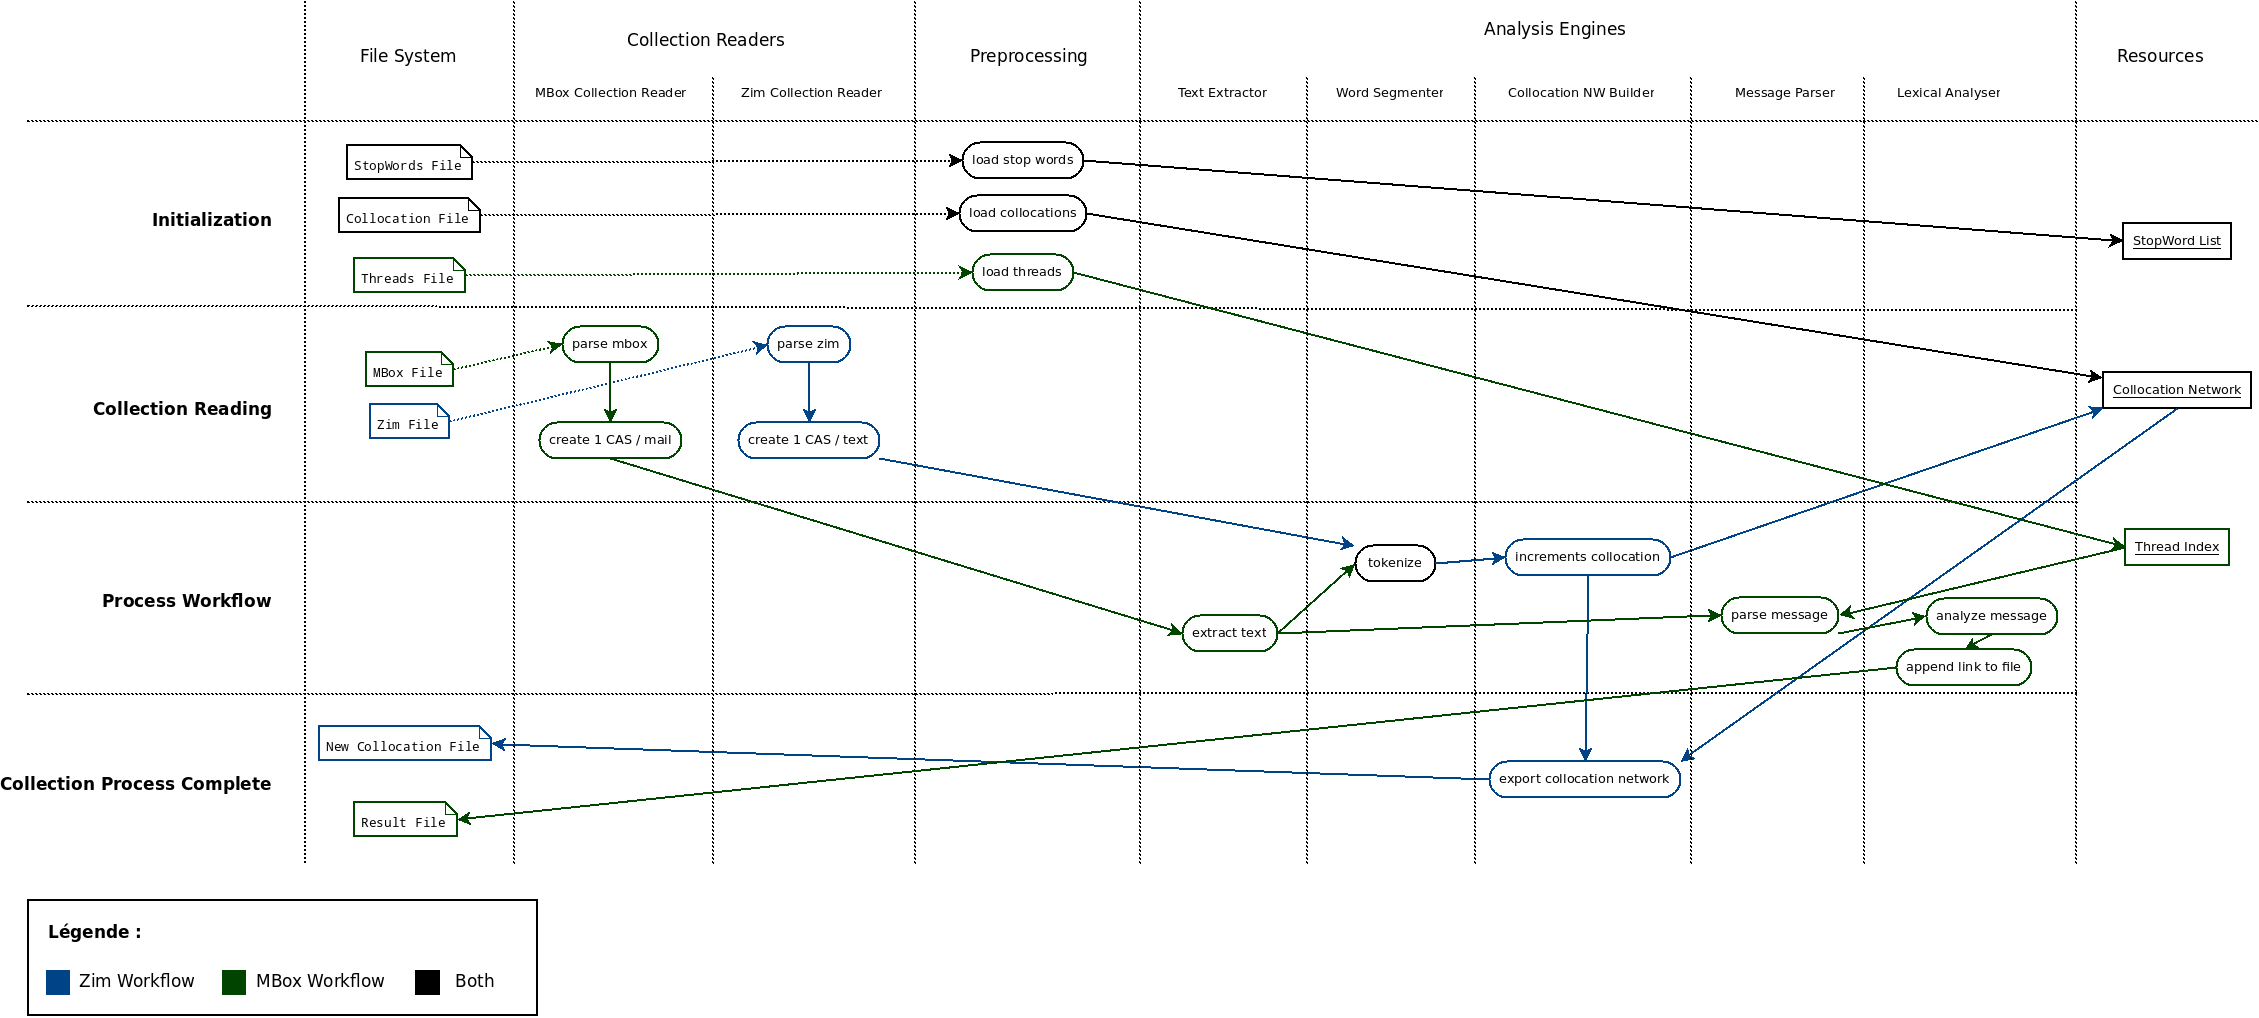
\includegraphics[width=\textwidth]{./uima-as_activity_diagram.png}
\label{overflow}
\end{figure}

Le fichier \texttt{uima-as\_activity\_diagram.png} représente le diagramme d'activité d'une hypothétique implémentation du programme avec UIMA AS. Il peut être consulté ou téléchargé dans sa version large à l'adresse suivante :\newline

\url{https://raw.github.com/bolaft/message-link-detector/master/uima-as_activity_diagram.png}

\subsection{Sources}

Les sources du programme peuvent être récupérées à l'adresse suivante :\newline

\url{https://github.com/bolaft/message-link-detector}

\end{document}